\chapter{Introduction}
\label{cha:chapter 1}
Autonomous vehicles (AV) have been a science fiction topic since their very first invention, however in the last years it started to evolve to a point where these will be seen in a early future driving in our streets. Big technology companies such as Google and Tesla compete not only between them, but with established car companies like Mercedes Benz, Nissan, Ferrari, Lamborghini and many others due to the investment of this particular area. Nevertheless, that does not mean research centers are not involved developing their own prototypes \cite{ModellingAutonomousVehicles}. Since the outcome of scale models along new technologies the limitation of having a car exclusively for experiments was overcome making possible to almost any research center to work in the autonomous vehicles interest.The purpose of this research is to make a full autonomous vehicle capable of driving and parking in a specific environment according to the Torneo Mexicano de Robotica (TMR) which has a category of AutoModelCar organized by Federacion Mexicana de Robotica; at moment the objectives are based in such category\cite{AutoModelCarRuleBook2019} as a bridge to develop a full scale car in order to drive by themselves in a real environment. This paper will address current progress particularly to the AutoNOMOS  mini, a vehicle model (scale 1:10 shown in the Figure \ref{fig:AutoNOMOS_mini}) owned by the Instituto Nacional de Astrofísica, Óptica y Electrónica (INAOE) by the Robotics Team. The AutoNOMOS mini runs Linux Ubuntu 14.04 and Robotic Operating System (ROS) on the top in a ODROID-XU4 64GB, this last one allows the vehicle to identify obstacles, rails, position using a , and perform different tasks using different sensors such as depth camera, laser RPLidar drive regardless of encountering obstacles or not thanks to the depth camera which gives the recognition of lanes and detection of obstacles along with sensors installed in the chassis.
\begin{figure}[h]
    \centering
    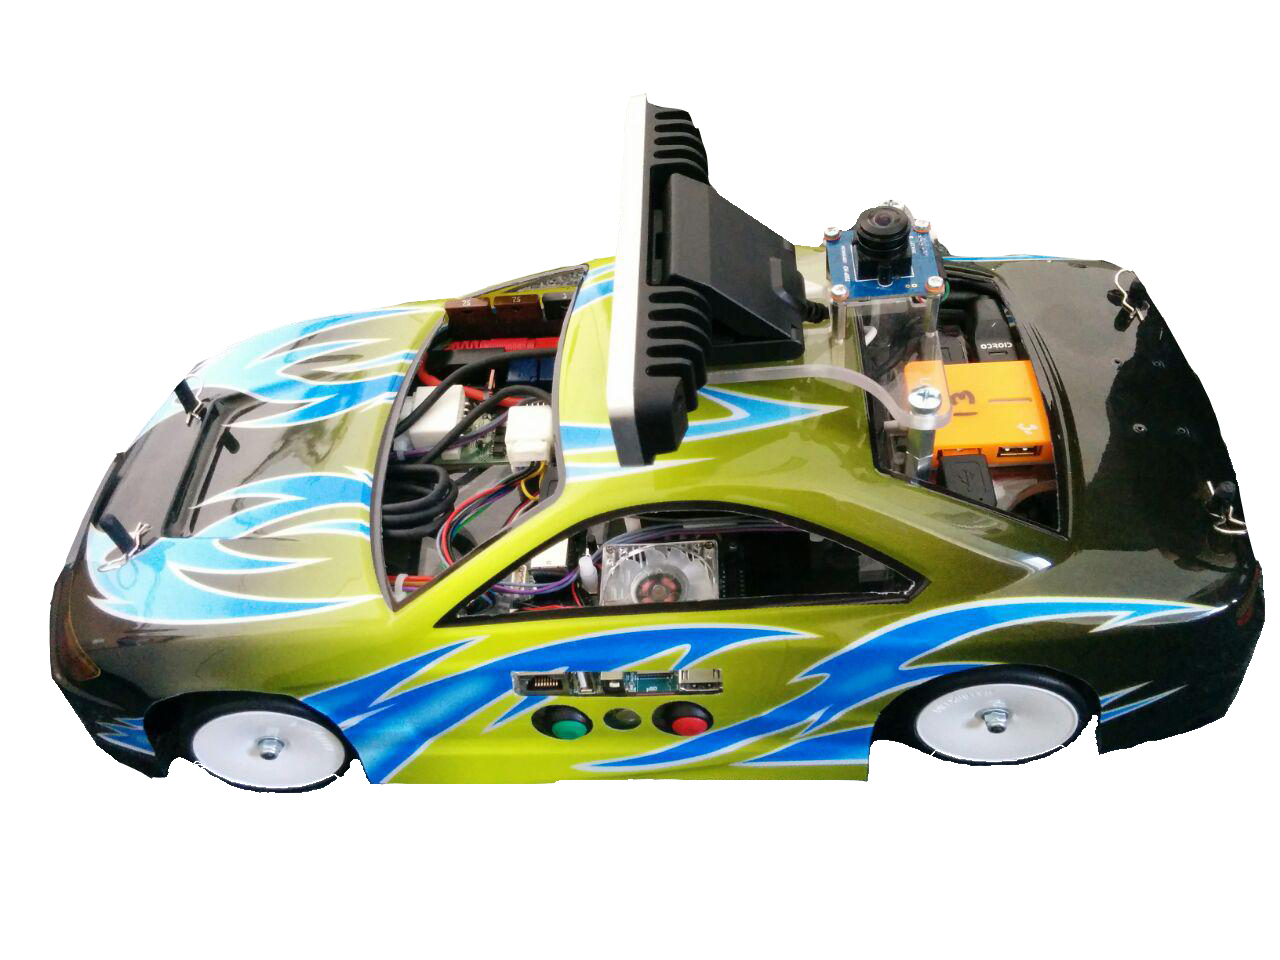
\includegraphics[width=6cm]{Figures/AutoNOMOS.jpg} \\[2mm]
    \caption{AutoNOMOS mini}
    \label{fig:AutoNOMOS_mini}
\end{figure}

\section{Background}
    \subsection{History}
    Ever since the very first car was created, science fiction comics has been keeping the expectation of driver-less cars, taxis, trucks in their pages since 1935 making it the as the first contact to AV. General Motors exhibit Futurama, "Highways and Horizons", in 1939 at New York World's Fair where predicted AV by magnetic trails built into the road's surface, or physical slots, or train-like rails keeping the car in their own "track", but this meant that roads and the structure had to be re-designed not only in a small part of the city, but all around the country. Even if the predicted project was a success, the investment to re-design the highways and roads it's expensive making it no good-looking for investors.\\
    \\In 1980s, Ernst Dickmans, working along with a team at Bundeswehr University Munich pioneered the very first practical driver-less technology with a Mercedes van; this van could drive up to 110mph  on traffic-free streets without any road side infrastructure required unlike GM suggested back in 1939. By 1989, the van was able to recognize obstacles, but it wasn't until the 1990s when was able to perform lane change autonomously.\\
    \\By the 2000s, several companies, universities and research labs, sparked their desire to get involved into the AV development thanks to this very first demonstration of a functional driver-less car. However, Defense  Advanced  Research  Projects  Administration  (DARPA) launch "Grand Challenge" where teams were challenged to complete a 150km off road and unmarked route in the Mojave desert; the idea was to stimulate the innovation of AV through this contest having a price of \$1m. The first edition of the contest in 2004 had no winners, having the vehicles driving few miles before crashing. Nevertheless, in 2005 DARPA held another challenge raising the prize to \$2m since the challenge itself had more obstacles and turns, this time Standford University won with a modified Volkswagen Tourag, a total of five out of the twenty-three teams completed the circuit with nary a scratch. In the following year, DARPA held a third edition of the challenge with new rules such as comply the with traffic laws, to respond to traffic and obstacles. Carnegie Mellon University with a modified Chevrolet Tahoe\cite{DARPA}.
    
    \subsection{Automation Levels}
    Fully autonomous cars and trucks that drive instead of people will become a reality in a not so distant future. As the technology progress this AV will being incorporated to the roads as they progress through levels of driving assistance technology. The National Highway Traffic Safety Administration (NHTSA) classified (taken directly from NHTSA 2020) the progress of this technology in six levels from no automation to full autonomy \cite{nhtsa}:
    \begin{itemize}
        \item Level 0: The human driver does all the driving.
        \item Level 1: An advanced driver assistance system (ADAS) on the vehicle can sometimes assist the human driver with either steering or braking/accelerating, but not both simultaneously.
        \item Level 2: An advanced driver assistance system (ADAS) on the vehicle can itself actually control both steering and braking/accelerating simultaneously under some circumstances.  The human driver must continue to pay full attention (“monitor the driving environment”) at all times and perform the rest of the driving task.
        \item Level 3: 	An Automated Driving System (ADS) on the vehicle can itself perform all aspects of the driving task under some circumstances.  In those circumstances, the human driver must be ready to take back control at any time when the ADS requests the human driver to do so.  In all other circumstances, the human driver performs the driving task.
        \item Level 4: 	An Automated Driving System (ADS) on the vehicle can itself perform all driving tasks and monitor the driving environment – essentially, do all the driving – in certain circumstances.  The human need not pay attention in those circumstances.
        \item Level 5: 	An Automated Driving System (ADS) on the vehicle can do all the driving in all circumstances.  The human occupants are just passengers and need never be involved in driving.
    \end{itemize}
    
    \subsection{Issues to address}
    Even though AV had important technological achievements in the last years, they still facing particular problems that researchers and car industries must solve before AV can fully replace the driver in the public roads\cite{RAND}.\\
    \\Techonological problem as image recognition in the traffics lights still presenting issues in different environmental situations such as heavy rain, snow, hail, night making the prototypes unable yet to drive; this environmental problems not only affect the recognition, but the sensors may fail due to an electrical failure, physical constrains due to the weather. Algorithms are not fully prepared to identify when the sensors are not working properly, the reason is because is not easy to identify when a sensor update sporadic fake values.\\
    \\A common fear among the citizens since technology started to sprout its the digital security. When internet first was released to the public the nervousness to hackers started to being a reality since the security algorithms were not as advanced as nowadays, this caused a huge economical loss to banks, and people who had all their information in their computers. The same fear is shared with driver-less cars, allowing AV to connect to cloud services in order to update not only mapping, but behavior of the car, and either physical or electrical conditions. This is indeed a security risk to treat, hackers may cause not only public damages as lives in danger, but economical loss and interfere with the communication dedicated to upload updates in short and long communications.\\
    \\Drivers, and traffic workers or any other job associated to transportation do not totally agree with the changes coming for the future despite the social and traffic benefits which will be address later in the paper since this may cause not only getting them fired, but reducing the cost of insurances, maintenance and inspectors.\\
    
    \subsection{Benefits}
    Investors, politicians, researchers, car companies, and technology companies realize that AV research can not be stopped only due to the nonconformity of the citizens, in the other hand they believe and share their technological advances and how these will be beneficial to everyone rather than the popular believe.\\
    \\Its well know that car accidents its the biggest cause of deaths worldwide because the driver can not properly react when an obstacle appears in front of the car due to the nervous to crash. The human reaction depends on the condition, if its healthy, doesn't have any toxic substance in the body, the body its under alcohol effects and emotional behaviours. AV expect to reduce this causalities and save more lives, by automatic breaking as soon as the car detects an unpredictable obstacle reducing rear-end obstacles, and human error despite their condition.\\
    \\In the morning, afternoon, and night exists peak hours where the roads are overcrowded making it difficult to anyone drive fluently. This tends to happen since some drivers do not have the proper traffic education increasing crashes, and delays. Nowadays, Google already tells you which roads are most crowded in order to take another route. However, AV can reduce it because of a more efficient vehicle operation avoiding disasters and taking the best route to achieve the destiny.
    
\section{Problem Statement}
Although in the AV test the results show that are able to identify obstacles, traffic lights, lanes, and the environment most of those experiments are done in an almost perfect conditions this is due to the lack of experiments in a real environment in which can gather real data of how these technologies are progressing. AV are still facing problems such as navigation, position, and anomalies detection in a not controlled environment like in a city surrounded by different anomalies. Since the re-design of infrastructure to have specific roads for these AV is expensive and a long-term project which is not efficient, driver-less cars must be capable to identify, drive, avoid obstacles, and follow the route planned by either the GPS or a pre-programmed route without invading one lane of the opposite direction, unless its necessary, the lane free of obstacles (another vehicle), and allowed by the corresponding traffic laws. One of the biggest problems when driving even for experimented drivers its taking curves on narrow roads in highway and in the city.\\
\\The problem is address on a two-way road, it may contain crossroads depending on the space to be tested. No map is available, every decision has to be made as its running. The rail planning will be done by artificial vision. However, since the laboratory does not count with light reflection and patters the surface where the vehicle will be tested its the normal floor of a house which is sensible to light reflection and have patters causing problems at the moment of identifying the edges of the road. Due to the mechanical constrains the AutoNOMOS mini has an steering angle limitation of $\pm14.77$ degrees or 0.224 rad taking the y-axis as the reference, calculated with the Ackerman Steering geometry model, for more information see the Chapter \ref{cha:chapter 2}, its fundamental to understand the steering angle of the vehicle to identify and plan how the curves should be taken. One of the most common problems of the AV, its how easy perturbation can be added to the sensors used for feedback. 

\section{Justification}
Research centers, universities, and big companies are supporting the AV are aware that driving its a trend topic as new technology keeps coming out reason to research it as a way to ease people's transportation in their own vehicle, taking the bus, working as truckers, delivery, etc. It's well known latest cars have incorporated GPS, steering and parking guide, proximity sensors, but the driver is still taking the decisions based on the information given by the car. Nevertheless, accidents happens due to incorrect decisions by the drivers in spite of what the sensors gave shown, drivers think that their experience is good enough to overcome any situation but the truth its that humans are never prepared to face a possible accident, unless have a huge amount of experience otherwise an accident its inevitable. AV are meant to help drivers to overcome situations that are not suited for not well-experienced drivers to either avoiding accidents, taking a better route or taking correctly a curve. 

\section{Scope and limitations}
    \subsection{Circuit Zone}
    This study will focus on developing an algorithm capable to drive in specifics environments and stages used in the TMR as evaluation points. The final tests are aimed to be realized in an black artificial plastic mat with 12x8m dimensions similar used in the TMR contests, in case of not counting with a carpet with the desired dimensions the circuit will be re-designed to fit in the obtained one. In the Figure \ref{fig:Track} shows the circuit used in the competences with an expected light reflection. The external, the inner and the dotted line radius have a value of 1.8m, 1m and 1.4m respectively. The wide of each rail its 40cm.
    \begin{figure}[h]
        \centering
        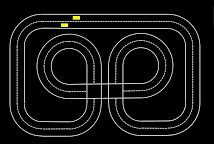
\includegraphics[width=12cm]{Figures/pista.png} \\[2mm]
        \caption{Track 1200x800cm (x,y)}
        \label{fig:Track}
    \end{figure}
    
    \subsection{Parking Zone}
    Separated from the circuit zone, exists a parking zone for the tests with regulations according with the size of the vehicle as shown in the Figure \ref{fig:ParkingZone}. The obstacles and the sidewalk are simulated by "walls" tall enough to be detected by the sensors in the vehicle.
    \begin{figure}[h]
        \centering
        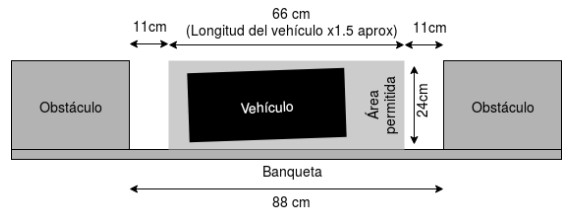
\includegraphics[width=10cm]{Figures/parking zone.PNG} \\[2mm]
        \caption{Parking Zone}
        \label{fig:ParkingZone}
    \end{figure}
    
    \subsection{Limitations}
    There are limitations that the vehicle AutoNOMOS mini must follow taken by the TMR rules\cite{AutoModelCarRuleBook2019}:
    \begin{itemize}
        \item Under no circumstance the vehicle can not be controlled remotely. The navigation must be autonomous and the only moment where the "driver" can act its to prepare the the initial boot or when the car must be stopped, due to any possible collision.
        \item All the process must be done in the vehicle. However, an external device can be used only to visualize the information of the vehicle and the emergency stop.
        \item The initial pose (position and direction) must be different in all the tests done.
        \item If the vehicle crash with an obstacle within the circuit the test will end immediately.
    \end{itemize}

\section{Objectives}
    \subsection {General}
    The aim of the AutoNOMOS mini platform is to drive in a circuit with either static or dynamic obstacles in different points of the map without leaving the rail where it was placed when started the tests. Since the idea its to develop an AV this have to be capable to park just as specified in the traffic regulations.
    
    \subsection {Specific}
    There are four specific objectives that the vehicle must perform, each test has a different level of difficulty:
    \begin{enumerate}
        \item \textbf{Autonomous Navigation without obstacles}\\ The vehicle must navigate in the circuit from the beginning to the end without leaving the rail.
        \item \textbf{Autonomous Navigation with obstacles}\\ The vehicle must navigate with obstacles (white boxes) around the circuit.
        \item \textbf{Autonomous navigation with mobile obstacles, following and overtaking}\\ The vehicle must navigate with two static obstacles and one dynamic ( a white box manually controlled by an external person simulating another vehicle). The vehicle must reduce its velocity to follow the obstacle and only when this one stops, the car can overtake it.
        \item \textbf{Autonomous Parking}\\ The vehicle must be able to park in the parking zone shown in the Figure \ref{fig:ParkingZone}. The vehicle must start with one meter of distant from the zone.
    \end{enumerate}
In the TMR rules the objectives have to be realized within 10 minutes. However, in this study there are not limit time to perform and finish the tests.